\section{Method and System Architecture}
\label{sec:method}

\critical comprises three coupled stages: (1)~diverse-perceiver measurement, (2)~adversarial feature discovery with independent media grounding, and (3)~calibrated fusion and selective prediction (Figure~\ref{fig:flowchart}; core notation in Table~\ref{tab:notation}). Given an editing instruction and two candidate videos with canonical identities $A$ and $B$ (invariant to display position), each stage transforms multimodal observations into versioned, inspectable records. Offline calibration fits parameters against human preference targets $y_i\in[0,1]$ on source-disjoint groups, while inference-time model requests receive only the instruction and permitted media without $y_i$ or target-revealing metadata.

\begin{figure*}[t]
\centering
% Approved CritiCal system overview: direction A (parallel evidence paths).
% Native TikZ; see input-example-provenance.txt for illustrative thumbnail source.
\begingroup
\definecolor{criticalEFF5F9}{HTML}{EFF5F9}
\definecolor{criticalC7D0D6}{HTML}{C7D0D6}
\definecolor{critical246083}{HTML}{246083}
\definecolor{criticalEEF6F2}{HTML}{EEF6F2}
\definecolor{critical23675B}{HTML}{23675B}
\definecolor{criticalF7F8FA}{HTML}{F7F8FA}
\definecolor{critical202830}{HTML}{202830}
\definecolor{criticalFFFFFF}{HTML}{FFFFFF}
\definecolor{critical56616B}{HTML}{56616B}
\definecolor{critical8A5824}{HTML}{8A5824}
\resizebox{0.84\textwidth}{!}{%
\begin{tikzpicture}[x=1pt,y=-1pt]
\path[use as bounding box] (0,20) rectangle (1440,558);
\path[fill=criticalEFF5F9,draw=criticalC7D0D6,line width=1.6pt,rounded corners=8pt] (230,22.5) rectangle (730,247.5);
\node[anchor=base west,inner sep=0pt,outer sep=0pt,text=critical246083,font={\sffamily\fontsize{25}{30.5}\selectfont\bfseries}] at (248,53.1) {1  Diverse-perceiver measurement};
\path[fill=criticalEEF6F2,draw=criticalC7D0D6,line width=1.6pt,rounded corners=8pt] (230,297) rectangle (730,499.5);
\node[anchor=base west,inner sep=0pt,outer sep=0pt,text=critical23675B,font={\sffamily\fontsize{25}{30.5}\selectfont\bfseries}] at (248,327.6) {2  Adversarial feature discovery};
\path[fill=criticalF7F8FA,draw=criticalC7D0D6,line width=1.6pt,rounded corners=8pt] (755,22.5) rectangle (1420,499.5);
\node[anchor=base west,inner sep=0pt,outer sep=0pt,text=critical202830,font={\sffamily\fontsize{25}{30.5}\selectfont\bfseries}] at (773,53.1) {3  Calibrated decision routing};
% Concrete input example; the two AI-generated halves are clipped natively.
\path[fill=criticalFFFFFF,draw=critical202830,line width=1.6pt,rounded corners=5pt] (15,96) rectangle (180,526);
\node[anchor=base,inner sep=0pt,outer sep=0pt,text=critical202830,font={\sffamily\fontsize{22}{26.84}\selectfont\bfseries}] at (97.5,129) {Instruction};
\node[anchor=base,inner sep=0pt,outer sep=0pt,text=critical202830,font={\sffamily\fontsize{20}{24.4}\selectfont}] at (97.5,156) {Show pink-dress};
\node[anchor=base,inner sep=0pt,outer sep=0pt,text=critical202830,font={\sffamily\fontsize{20}{24.4}\selectfont}] at (97.5,180) {making in steps.};
\node[anchor=base west,inner sep=0pt,outer sep=0pt,text=critical202830,font={\sffamily\fontsize{21}{25.62}\selectfont\bfseries}] at (25,211) {Video A};
\begin{scope}
\clip (25,224) rectangle (170,332.75);
\node[anchor=north west,inner sep=0pt,outer sep=0pt] at (25,224) {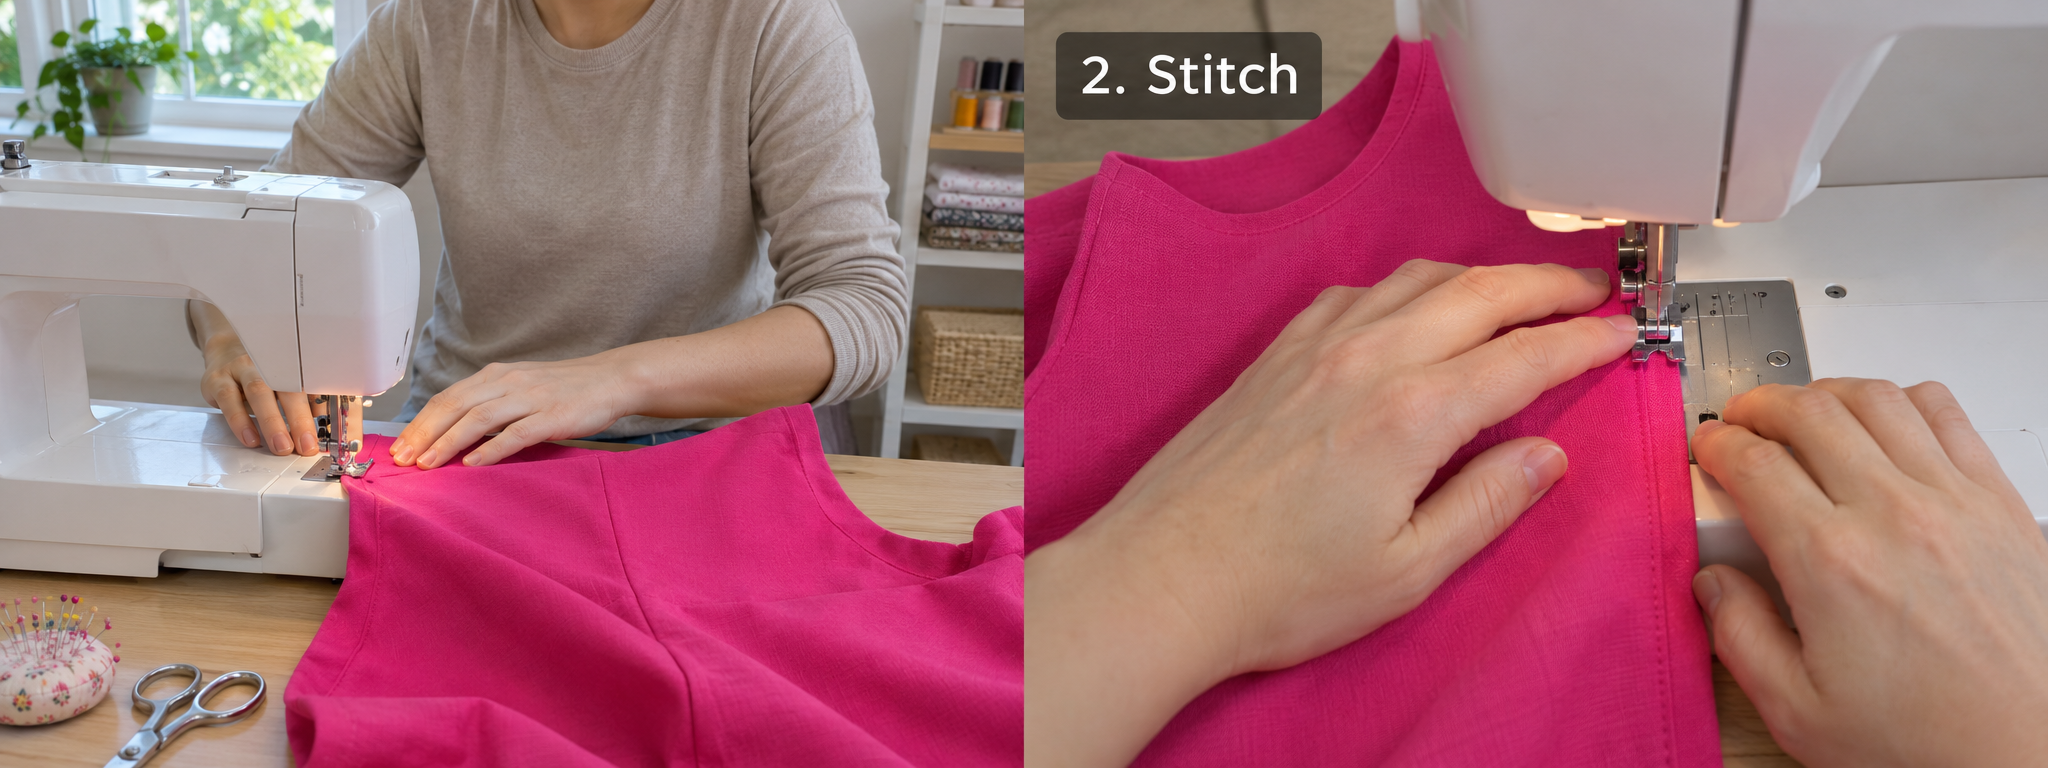
\includegraphics[width=290pt]{figures/flowchart/input-example-pair.png}};
\end{scope}
\node[anchor=base west,inner sep=0pt,outer sep=0pt,text=critical202830,font={\sffamily\fontsize{21}{25.62}\selectfont\bfseries}] at (25,357) {Video B};
\begin{scope}
\clip (25,370) rectangle (170,478.75);
\node[anchor=north west,inner sep=0pt,outer sep=0pt] at (-120,370) {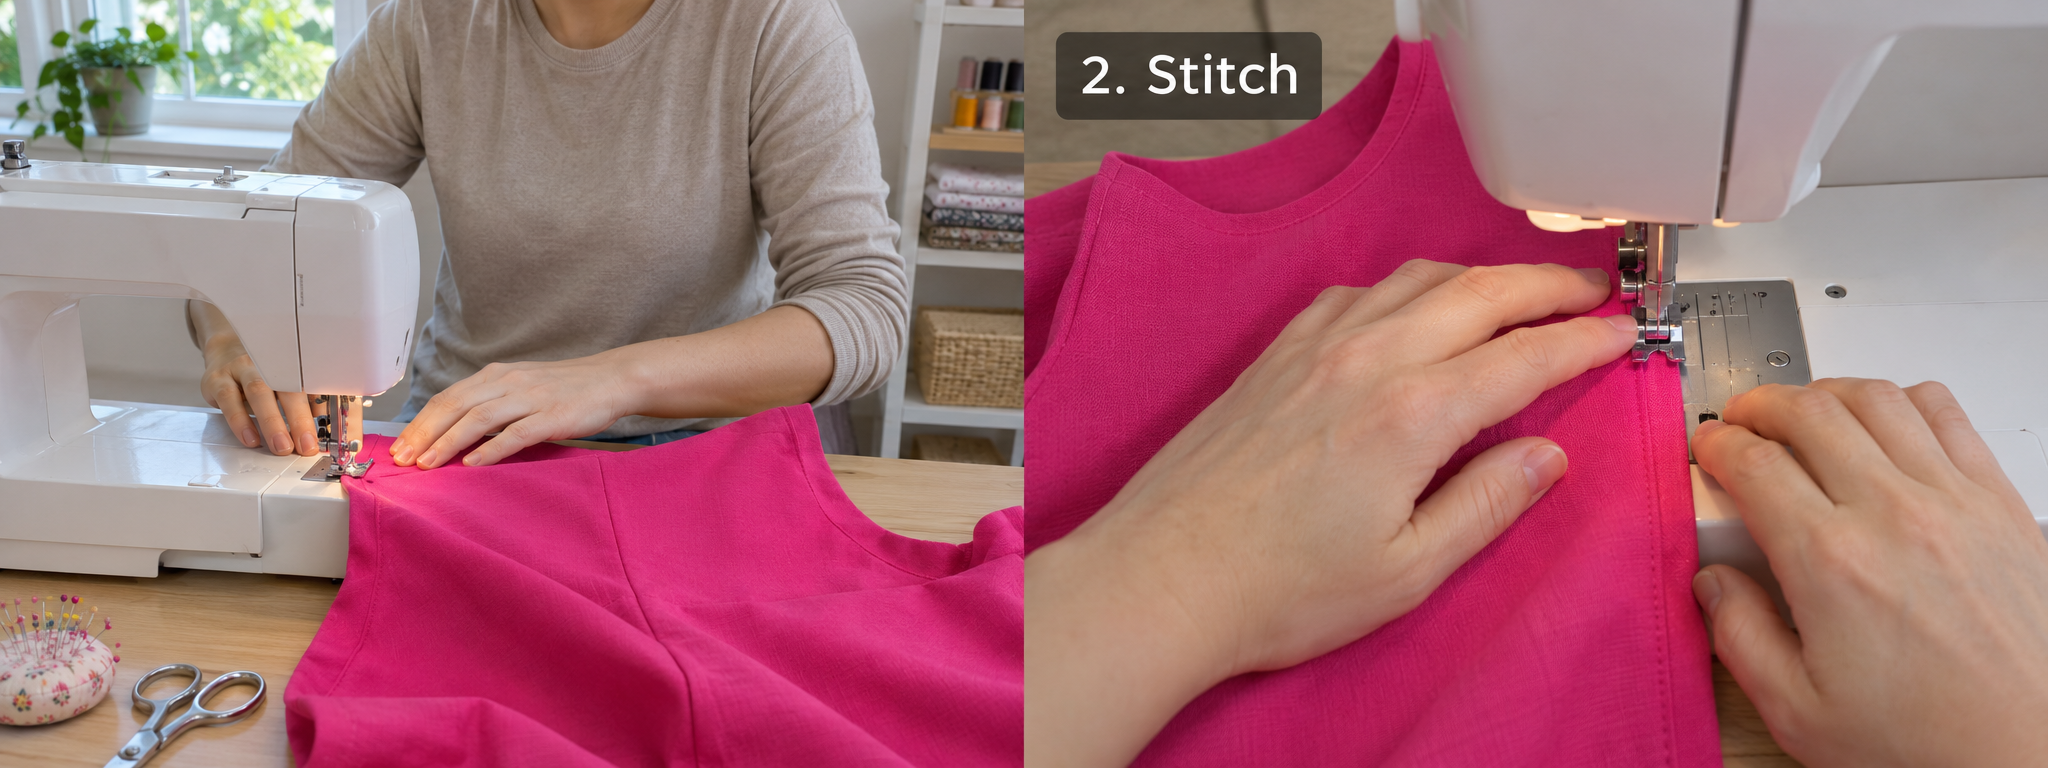
\includegraphics[width=290pt]{figures/flowchart/input-example-pair.png}};
\end{scope}
\node[anchor=base,inner sep=0pt,outer sep=0pt,text=critical56616B,font={\sffamily\fontsize{20}{24.4}\selectfont}] at (97.5,511) {Illustrative frames};
\draw[draw=critical202830,line width=2pt,line join=round,-{Stealth[length=8pt,width=8pt]}] (180,283.5) -- (205,283.5) -- (205,108.9) -- (250,108.9);
\draw[draw=critical202830,line width=2pt,line join=round,-{Stealth[length=8pt,width=8pt]}] (205,189.9) -- (250,189.9);
\draw[draw=critical202830,line width=2pt,line join=round,-{Stealth[length=8pt,width=8pt]}] (205,283.5) -- (205,405) -- (250,405);
\path[fill=criticalFFFFFF,draw=critical246083,line width=1.6pt,rounded corners=5pt] (250,78.3) rectangle (475,139.5);
\node[anchor=base,inner sep=0pt,outer sep=0pt,text=critical246083,font={\sffamily\fontsize{23}{28.06}\selectfont\bfseries}] at (362.5,101.745) {Native-video};
\node[anchor=base,inner sep=0pt,outer sep=0pt,text=critical56616B,font={\sffamily\fontsize{21}{25.62}\selectfont}] at (362.5,130.545) {Temporal / audio};
\path[fill=criticalFFFFFF,draw=critical246083,line width=1.6pt,rounded corners=5pt] (250,159.3) rectangle (475,220.5);
\node[anchor=base,inner sep=0pt,outer sep=0pt,text=critical246083,font={\sffamily\fontsize{23}{28.06}\selectfont\bfseries}] at (362.5,182.745) {Frame-based};
\node[anchor=base,inner sep=0pt,outer sep=0pt,text=critical56616B,font={\sffamily\fontsize{21}{25.62}\selectfont}] at (362.5,211.545) {Timestamped frames};
\path[fill=criticalFFFFFF,draw=critical246083,line width=1.6pt,rounded corners=5pt] (520,94.5) rectangle (710,211.5);
\node[anchor=base,inner sep=0pt,outer sep=0pt,text=critical246083,font={\sffamily\fontsize{24}{29.28}\selectfont\bfseries}] at (615,121.428) {Canonical};
\node[anchor=base,inner sep=0pt,outer sep=0pt,text=critical246083,font={\sffamily\fontsize{24}{29.28}\selectfont\bfseries}] at (615,147.78) {consensus};
\node[anchor=base,inner sep=0pt,outer sep=0pt,text=critical56616B,font={\sffamily\fontsize{21}{25.62}\selectfont}] at (615,177.48) {AB / BA judgments};
\node[anchor=base,inner sep=0pt,outer sep=0pt,text=critical56616B,font={\sffamily\fontsize{21}{25.62}\selectfont}] at (615,200.538) {Stability + criteria};
\draw[draw=critical202830,line width=2pt,line join=round,-{Stealth[length=8pt,width=8pt]}] (475,108.9) -- (496,108.9) -- (496,134.1) -- (520,134.1);
\draw[draw=critical202830,line width=2pt,line join=round,-{Stealth[length=8pt,width=8pt]}] (475,189.9) -- (496,189.9) -- (496,172.8) -- (520,172.8);
\path[fill=criticalFFFFFF,draw=critical23675B,line width=1.6pt,rounded corners=5pt] (250,360) rectangle (380,450);
\node[anchor=base,inner sep=0pt,outer sep=0pt,text=critical23675B,font={\sffamily\fontsize{22}{26.84}\selectfont\bfseries}] at (315,399.258) {Advocate A};
\node[anchor=base,inner sep=0pt,outer sep=0pt,text=critical23675B,font={\sffamily\fontsize{22}{26.84}\selectfont\bfseries}] at (315,423.414) {Advocate B};
\path[fill=criticalFFFFFF,draw=critical23675B,line width=1.6pt,rounded corners=5pt] (408,360) rectangle (553,450);
\node[anchor=base,inner sep=0pt,outer sep=0pt,text=critical23675B,font={\sffamily\fontsize{21}{25.62}\selectfont\bfseries}] at (480.5,399.519) {Independent};
\node[anchor=base,inner sep=0pt,outer sep=0pt,text=critical23675B,font={\sffamily\fontsize{21}{25.62}\selectfont\bfseries}] at (480.5,422.577) {referee};
\path[fill=criticalFFFFFF,draw=critical23675B,line width=1.6pt,rounded corners=5pt] (580,360) rectangle (710,450);
\node[anchor=base,inner sep=0pt,outer sep=0pt,text=critical23675B,font={\sffamily\fontsize{22}{26.84}\selectfont\bfseries}] at (645,399.258) {Factors};
\node[anchor=base,inner sep=0pt,outer sep=0pt,text=critical23675B,font={\sffamily\fontsize{22}{26.84}\selectfont\bfseries}] at (645,423.414) {+ evidence};
\draw[draw=critical202830,line width=2pt,line join=round,-{Stealth[length=8pt,width=8pt]}] (380,405) -- (408,405);
\draw[draw=critical202830,line width=2pt,line join=round,-{Stealth[length=8pt,width=8pt]}] (553,405) -- (580,405);
\node[anchor=base west,inner sep=0pt,outer sep=0pt,text=critical56616B,font={\sffamily\fontsize{21}{25.62}\selectfont}] at (251,482.4) {Referee independently re-inspects permitted media};
\path[fill=criticalFFFFFF,draw=critical202830,line width=1.6pt,rounded corners=5pt] (780,337.5) rectangle (1005,468);
\node[anchor=base,inner sep=0pt,outer sep=0pt,text=critical202830,font={\sffamily\fontsize{24}{29.28}\selectfont\bfseries}] at (892.5,372.825) {Calibration features};
\node[anchor=base,inner sep=0pt,outer sep=0pt,text=critical56616B,font={\sffamily\fontsize{21}{25.62}\selectfont}] at (892.5,402.525) {Preferences + criteria};
\node[anchor=base,inner sep=0pt,outer sep=0pt,text=critical56616B,font={\sffamily\fontsize{21}{25.62}\selectfont}] at (892.5,425.583) {Instability + masks};
\node[anchor=base,inner sep=0pt,outer sep=0pt,text=critical56616B,font={\sffamily\fontsize{21}{25.62}\selectfont}] at (892.5,448.641) {Grounded factors};
\draw[draw=critical202830,line width=2pt,line join=round,-{Stealth[length=8pt,width=8pt]}] (710,153) -- (744,153) -- (744,367.2) -- (780,367.2);
\draw[draw=critical202830,line width=2pt,line join=round,-{Stealth[length=8pt,width=8pt]}] (710,405) -- (780,405);
\path[fill=criticalFFFFFF,draw=critical246083,line width=1.6pt,rounded corners=5pt] (780,112.5) rectangle (1005,225);
\node[anchor=base,inner sep=0pt,outer sep=0pt,text=critical246083,font={\sffamily\fontsize{25}{30.5}\selectfont\bfseries}] at (892.5,148.446) {Fusion +};
\node[anchor=base,inner sep=0pt,outer sep=0pt,text=critical246083,font={\sffamily\fontsize{25}{30.5}\selectfont\bfseries}] at (892.5,175.896) {calibration};
\node[anchor=base,inner sep=0pt,outer sep=0pt,text=critical56616B,font={\sffamily\fontsize{21}{25.62}\selectfont}] at (892.5,206.496) {P(A preferred to B)};
\draw[draw=critical202830,line width=2pt,line join=round,-{Stealth[length=8pt,width=8pt]}] (893,337.5) -- (893,225);
\path[fill=criticalFFFFFF,draw=critical202830,line width=1.6pt,rounded corners=5pt] (1040,112.5) rectangle (1195,225);
\node[anchor=base,inner sep=0pt,outer sep=0pt,text=critical202830,font={\sffamily\fontsize{24}{29.28}\selectfont\bfseries}] at (1117.5,148.707) {Reliability};
\node[anchor=base,inner sep=0pt,outer sep=0pt,text=critical202830,font={\sffamily\fontsize{24}{29.28}\selectfont\bfseries}] at (1117.5,175.059) {gate};
\node[anchor=base,inner sep=0pt,outer sep=0pt,text=critical56616B,font={\sffamily\fontsize{21}{25.62}\selectfont}] at (1117.5,204.759) {Risk signals};
\draw[draw=critical202830,line width=2pt,line join=round,-{Stealth[length=8pt,width=8pt]}] (1005,168.3) -- (1040,168.3);
\draw[draw=critical202830,line width=2pt,line join=round,-{Stealth[length=8pt,width=8pt]}] (1005,405) -- (1020,405) -- (1020,202.5) -- (1040,202.5);
\node[anchor=base,inner sep=0pt,outer sep=0pt,text=critical56616B,font={\sffamily\fontsize{21}{25.62}\selectfont}] at (1118,315) {Order instability};
\node[anchor=base,inner sep=0pt,outer sep=0pt,text=critical56616B,font={\sffamily\fontsize{21}{25.62}\selectfont}] at (1118,338.058) {Disagreement};
\node[anchor=base,inner sep=0pt,outer sep=0pt,text=critical56616B,font={\sffamily\fontsize{21}{25.62}\selectfont}] at (1118,361.116) {Missing evidence};
\node[anchor=base,inner sep=0pt,outer sep=0pt,text=critical56616B,font={\sffamily\fontsize{21}{25.62}\selectfont}] at (1118,384.174) {Preference shift};
\path[fill=criticalFFFFFF,draw=critical23675B,line width=1.6pt,rounded corners=5pt] (1230,85.5) rectangle (1400,162);
\node[anchor=base,inner sep=0pt,outer sep=0pt,text=critical23675B,font={\sffamily\fontsize{25}{30.5}\selectfont\bfseries}] at (1315,117.171) {Accept};
\node[anchor=base,inner sep=0pt,outer sep=0pt,text=critical56616B,font={\sffamily\fontsize{21}{25.62}\selectfont}] at (1315,147.771) {Verdict + reason};
\path[fill=criticalFFFFFF,draw=critical8A5824,line width=1.6pt,rounded corners=5pt] (1230,220.5) rectangle (1400,297);
\node[anchor=base,inner sep=0pt,outer sep=0pt,text=critical8A5824,font={\sffamily\fontsize{25}{30.5}\selectfont\bfseries}] at (1315,252.171) {Investigate};
\node[anchor=base,inner sep=0pt,outer sep=0pt,text=critical56616B,font={\sffamily\fontsize{21}{25.62}\selectfont}] at (1315,282.771) {Call budget};
\path[fill=criticalFFFFFF,draw=critical202830,line width=1.6pt,rounded corners=5pt] (1230,355.5) rectangle (1400,432);
\node[anchor=base,inner sep=0pt,outer sep=0pt,text=critical202830,font={\sffamily\fontsize{25}{30.5}\selectfont\bfseries}] at (1315,387.171) {Defer};
\node[anchor=base,inner sep=0pt,outer sep=0pt,text=critical56616B,font={\sffamily\fontsize{21}{25.62}\selectfont}] at (1315,417.771) {Human / abstain};
\draw[draw=critical202830,line width=2pt,line join=round,-{Stealth[length=8pt,width=8pt]}] (1195,168.3) -- (1212,168.3) -- (1212,123.3) -- (1230,123.3);
\draw[draw=critical202830,line width=2pt,line join=round,-{Stealth[length=8pt,width=8pt]}] (1212,168.3) -- (1212,258.3) -- (1230,258.3);
\draw[draw=critical202830,line width=2pt,line join=round,-{Stealth[length=8pt,width=8pt]}] (1212,258.3) -- (1212,393.3) -- (1230,393.3);
\draw[draw=critical8A5824,line width=2pt,line join=round,dash pattern=on 8pt off 6pt,-{Stealth[length=8pt,width=8pt]}] (1400,258.3) -- (1410,258.3) -- (1410,553.5) -- (205,553.5) -- (205,283.5);
\node[anchor=base,inner sep=0pt,outer sep=0pt,text=critical8A5824,font={\sffamily\fontsize{23}{28.06}\selectfont}] at (800,541.8) {Bounded acquisition: frames, targeted criteria, or debate; validate and re-fuse};
\end{tikzpicture}%
}
\endgroup

\caption{\critical system overview across three stages: (1)~counterbalanced native-video and contact-sheet perceiver measurement, (2)~adversarial feature discovery with independent media-grounded referee verification, and (3)~statistical fusion and reliability-gated selective prediction.}
\Description{An illustrative instruction, Show pink-dress making in steps, and synthetic frames representing videos A and B feed native-video and frame-based perceivers in Stage 1 and opposing advocates plus an independent referee in Stage 2. A shows a medium sewing shot; B shows a close-up with a numbered step overlay. Canonical consensus and grounded factors feed fusion and a reliability gate in Stage 3 to accept, investigate, or defer. The frames are illustrative and do not depict a measured benchmark pair.}
\label{fig:flowchart}
\end{figure*}

\begin{table}[t]
\centering
\caption{Core notation used in \critical.}
\label{tab:notation}
\footnotesize
\begin{tabular}{@{}lp{5.5cm}@{}}
\toprule
Symbol & Meaning \\
\midrule
$A,\; B,\; y_i\in[0,1]$ & Canonical candidate identities and offline human vote fraction favoring $A$ on pair $i$. \\
$p^{AB}_{ij},\; p^{BA}_{ij}$ & Perceiver $j$'s left-preferred probability when $A$ or $B$ is shown first. \\
$\bar p_{ij},\; \iota_{ij}$ & Swap-averaged preference for $A$ and order-instability diagnostic (Eq.~\ref{eq:swap}). \\
$\phi_i,\; \beta,\; \hat p_i$ & Comparison feature vector, fitted calibration weights, and calibrated $P(A\succ B)$ (Eq.~\ref{eq:bt}). \\
$r_i,\; t_{\mathrm{accept}},\; t_{\mathrm{investigate}}$ & Reliability risk score and frozen decision-routing thresholds (Eq.~\ref{eq:route}). \\
\bottomrule
\end{tabular}
\end{table}

\subsection{Stage 1: Diverse-perceiver measurement}
\label{sec:perceivers}
Two native-video judges (e.g., Gemini-2.5-Pro and Gemini-3.7-Flash) share an accuracy ceiling when they perceive decoded video in the same way. \critical therefore pairs native-video perceivers with a \textbf{frame-based perceiver} that inspects a different representation so its errors are only weakly correlated with the video judges:
\begin{itemize}[leftmargin=*, topsep=2pt, itemsep=2pt]
  \item \textbf{Native-video perceivers} (e.g., Gemini-family video models) ingest the decoded video stream directly to evaluate temporal motion, pacing, transitions, and available audio, emitting structured rubric scores, timestamp-grounded evidence, and a pairwise preference probability.
  \item \textbf{Contact-sheet frame perceiver:} Scene-aware frame extraction and deduplication produce a timestamped $4\times 2$ contact sheet per clip~\cite{clauderealvideo}. An image-only VLM receives the two sheets side by side and emits the same structured judgment schema, with audio quality marked not applicable.
\end{itemize}

\paragraph{Counterbalanced judging and order stability.}
VLM judges frequently exhibit position bias, favoring whichever video is shown first. To factor this out, each perceiver $j$ evaluates the pair twice---once in display order $(A,B)$ and once in swapped order $(B,A)$. From the left-video preference probabilities $p^{AB}_{ij}$ and $p^{BA}_{ij}$, \critical computes the canonical preference for $A$ and an order-instability score:
\begin{equation}
\bar p_{ij}=\frac{p^{AB}_{ij}+(1-p^{BA}_{ij})}{2},
\qquad
\iota_{ij}=\bigl|p^{AB}_{ij}-(1-p^{BA}_{ij})\bigr|.
\label{eq:swap}
\end{equation}
Keeping $\iota_{ij}$ separates genuine indifference ($\bar p_{ij}\approx 0.5$ with low $\iota_{ij}$) from a position-biased flip ($\bar p_{ij}\approx 0.5$ with high $\iota_{ij}$). Alongside overall preference, each perceiver scores individual rubric criteria (instruction alignment, temporal consistency, visual quality, narrative coherence, and audio quality when applicable), yielding signed candidate differences and cross-perceiver disagreement signals.

\subsection{Stage 2: Adversarial debate and grounded factors}
\label{sec:debate}
Fixed rubric scores often fail on borderline video edits for two reasons: (1)~\emph{off-rubric criteria}, where the decisive factor is task-specific (e.g., instructional clarity for a classroom lesson) rather than a generic visual metric, and (2)~\emph{unchallenged surface impressions}, where a single-pass judge penalizes an apparent visual flaw without checking whether it is an intentional editing choice. To overcome both blind spots, \critical separates case generation from verification across three roles:
\begin{itemize}[leftmargin=*, topsep=2pt, itemsep=2pt]
  \item \textbf{Opposing advocates ($A$ vs.\ $B$):} Each agent is assigned one canonical candidate and must build the strongest timestamp-grounded case for its side while explicitly conceding undeniable weaknesses.
  \item \textbf{Independent referee:} Rather than letting persuasive rhetoric decide the winner, an independent referee inspects the competing arguments alongside the permitted media (including source videos when source preservation is disputed), verifies which claims hold up visually, and extracts the decisive contested factors.
\end{itemize}

\paragraph{Why multi-turn rebuttal matters (Figure~\ref{fig:factor-distillation}).}
When advocates only produce isolated monologues, they often talk past each other. A multi-turn exchange forces each side to test the other's visual evidence. Figure~\ref{fig:factor-distillation} illustrates this mechanism on a task asking an edit to \emph{explain flower types and lifespans to students}:
\begin{itemize}[leftmargin=*, topsep=2pt, itemsep=1pt]
  \item \textbf{Turn~1 (Surfacing task-specific criteria):} Advocate~$A$ identifies a task-specific advantage that a generic rubric misses---$A$'s bouquet shows multiple species side by side, making lifespan comparison more educational.
  \item \textbf{Turn~2 (Challenging visual evidence):} Advocate~$B$ attacks the visual quality of that exact shot, pointing out that $A$'s bouquet starts blurred whereas $B$'s single-flower close-up is immediately sharp.
  \item \textbf{Turn~3 (Disambiguating technique vs.\ defect):} Forced to respond to Turn~2, Advocate~$A$ re-examines the clip and explains that the initial blur is a deliberate focus pull that resolves cleanly, whereas $B$'s single-flower shot suffers from camera shake.
\end{itemize}

\paragraph{From debate transcript to structured calibration features.}
After the advocate turns conclude, the referee adjudicates the exchange and distills the dispute into structured \emph{factor records} rather than free-form text. Each factor stores a reusable label (e.g., \emph{educational value}, \emph{shot quality}), the favored canonical candidate ($\{-1,0,+1\}$), a referee-assessed decisiveness weight in $[0,1]$ (0.9 and 0.6 in Figure~\ref{fig:factor-distillation}), its mapping to a base rubric dimension, and timestamped supporting evidence. For downstream statistical fusion (Section~\ref{sec:fusion}), these records are summarized into a compact numerical block---comprising the referee's preference logit ($P(A)=0.85$ in the example), net signed factor lean, mean decisiveness, risk flags, and advocate concession asymmetry---along with an availability indicator in case a model call times out or fails schema validation.

\begin{figure}[t]
\centering
% Three-turn flowers pilot and terminal referee, grounded in flowers-debate-record.json.
\begingroup
\definecolor{fdInk}{HTML}{202830}
\definecolor{fdMuted}{HTML}{56616B}
\definecolor{fdGrey}{HTML}{C7D0D6}
\definecolor{fdBlue}{HTML}{246083}
\definecolor{fdGreen}{HTML}{23675B}
\definecolor{fdLight}{HTML}{F7F8FA}
\definecolor{fdBlueLight}{HTML}{EFF5F9}
\definecolor{fdGreenLight}{HTML}{EEF6F2}
\resizebox{\columnwidth}{!}{%
\begin{tikzpicture}[x=1pt,y=-1pt,
  fdtext/.style={anchor=north west,inner sep=0pt,outer sep=0pt,align=left,
    text=fdInk,font=\sffamily\fontsize{8}{9.4}\selectfont},
  fdhead/.style={fdtext,font=\sffamily\fontsize{8.2}{9.6}\selectfont\bfseries},
  fdsmall/.style={fdtext,text=fdMuted,font=\sffamily\fontsize{7}{8.2}\selectfont},
  fdcard/.style={line width=.55pt,rounded corners=4pt}
]
\path[use as bounding box] (0,0) rectangle (244,230);
\node[fdtext] at (0,0)
  {\textbf{Task:} explain flower types and lifespans to students.};
\node[fdhead] at (0,20) {Three debate turns};
\node[fdhead] at (168,20) {Distilled factors};
% Turn 1: A's opening.
\path[fdcard,draw=fdBlue,fill=fdBlueLight] (8,34) rectangle (158,73);
\path[draw=fdBlue,fill=fdBlueLight,line width=.55pt]
  (8,44) -- (2,49) -- (8,53);
\node[fdhead,text=fdBlue] at (15,38) {1\quad A: opening};
\node[fdtext,text width=136pt] at (15,51)
  {A's bouquet shows more species\newline for comparing lifespans.};
% Turn 2 explicitly challenges A's evidence.
\path[fdcard,draw=fdGreen,fill=fdGreenLight] (0,80) rectangle (150,119);
\path[draw=fdGreen,fill=fdGreenLight,line width=.55pt]
  (150,90) -- (156,95) -- (150,99);
\node[fdhead,text=fdGreen] at (7,84) {2\quad B: challenge};
\node[fdtext,text width=136pt] at (7,97)
  {That bouquet starts blurred.\newline B's single-flower shot is clearer.};
% Turn 3 answers the challenge rather than repeating the opening.
\path[fdcard,draw=fdBlue,fill=fdBlueLight] (8,126) rectangle (158,165);
\path[draw=fdBlue,fill=fdBlueLight,line width=.55pt]
  (8,136) -- (2,141) -- (8,145);
\node[fdhead,text=fdBlue] at (15,130) {3\quad A: rebuttal};
\node[fdtext,text width=136pt] at (15,143)
  {It's a focus pull that resolves.\newline B's single-flower shot is shaky.};
% Referee acts once after the debate, with no intervening questions.
\path[fdcard,draw=fdInk,fill=fdLight] (0,173) rectangle (158,214);
\node[fdhead] at (7,178) {Referee: final judgment};
\node[fdtext,text width=144pt] at (7,191)
  {Prefer A: more educational;\newline the focus pull is intentional.};
% Saved factor direction and decisiveness, not preference probabilities.
\path[fdcard,draw=fdGrey,fill=fdLight] (168,34) rectangle (244,165);
\node[fdhead,text width=64pt] at (174,40) {Educational\newline value};
\node[fdtext,text=fdBlue] at (174,64) {Favors A};
\node[fdsmall] at (174,77) {Importance 0.9};
\draw[draw=fdGrey,line width=.45pt] (174,97) -- (238,97);
\node[fdhead] at (174,106) {Shot quality};
\node[fdtext,text=fdBlue] at (174,121) {Favors A};
\node[fdsmall] at (174,136) {Importance 0.6};
\path[fdcard,draw=fdInk,fill=white] (168,173) rectangle (244,214);
\node[fdsmall] at (174,179) {Referee reports};
\node[fdhead] at (174,194) {$P(A)=0.85$};
\node[fdsmall] at (0,222)
  {Importance = referee-rated decisiveness (0--1), not probability.};
\end{tikzpicture}%
}
\endgroup

\caption{Multi-turn adversarial debate and factor distillation on an instructional flower-editing comparison. Three responsive advocate turns are adjudicated by the referee into structured factor weights and a preference probability.}
\Description{Turn 1: A favors a bouquet for its educational variety. Turn 2: B challenges its initial blur and favors a clearer single-flower shot. Turn 3: A identifies an intentional focus pull and contrasts B's shaky shot. The final referee favors A for educational value, importance 0.9, and shot quality, importance 0.6, and reports preference probability 0.85 for A. The referee adjudicates after the three advocate turns rather than steering between them.}
\label{fig:factor-distillation}
\end{figure}

\subsection{Stage 3a: Statistical fusion and calibration}
\label{sec:fusion}
Simple majority voting or score averaging treats every perceiver and every rubric dimension as equally trustworthy, even when one judge is unstable across display orders or blind to a modality. Instead, \critical stacks all signals from Stage~1 (Section~\ref{sec:perceivers}) and Stage~2 (Section~\ref{sec:debate}) into a single feature vector $\phi_i$ and learns how strongly each signal predicts human preference:
\begin{itemize}[leftmargin=*, topsep=2pt, itemsep=1pt]
  \item \textbf{Directional preference signals} (positive favors $A$, negative favors $B$): each perceiver's swap-averaged preference logit $\operatorname{logit}(\bar p_{ij})$, signed rubric-criterion differences between $A$ and $B$, and the referee's verified factor scores from Stage~2 (Section~\ref{sec:debate}).
  \item \textbf{Diagnostic and missingness signals:} order instability $\iota_{ij}$, cross-perceiver disagreement, and explicit binary missingness masks (so an unmeasured modality, such as audio on a frame-only judge, is never mistaken for a zero score).
\end{itemize}
Given $\phi_i$, \critical predicts the calibrated human preference probability via a logistic linear model:
\begin{equation}
\hat p_i = P(A\succ B\mid \phi_i,\beta)=\sigma(\beta^\top\phi_i),\qquad
\sigma(z)=(1+e^{-z})^{-1}.
\label{eq:bt}
\end{equation}

\paragraph{Two lightweight calibration heads.}
Because human preference datasets are often modest in size, $\beta$ must be regularized to avoid overfitting. \critical supports two lightweight fitting options depending on the task:
\begin{itemize}[leftmargin=*, topsep=2pt, itemsep=2pt]
  \item \textbf{Bayesian Bradley--Terry head (for swap-symmetric, small-sample calibration):} Uses only the directional difference features (with no intercept, so swapping $A$ and $B$ exactly flips $\hat p_i$ to $1-\hat p_i$). It fits $\beta$ against soft human vote fractions $y_i\in[0,1]$ under Gaussian priors and uses the local parameter uncertainty around $\hat\beta$ to temper overconfident predictions on unusual feature combinations.
  \item \textbf{Regularized expert-router head (for multi-perceiver fusion):} Combines all perceiver logits, criterion differences, stability/disagreement diagnostics, and Stage~2 debate features (Section~\ref{sec:debate}) in an $L_2$-regularized logistic stacker trained on majority human preferences. This is the head used by the unified \critical router in Section~\ref{sec:evaluation}.
\end{itemize}
In both cases, feature normalization and weights $\beta$ are fitted strictly on source-disjoint training groups, and held-out evaluations use grouped out-of-fold predictions so human labels never leak into inference.

\subsection{Stage 3b: Reliability gate and selective prediction}
\label{sec:gate}
Predicting \emph{which} video is better ($\hat p_i$) is not the same as knowing \emph{whether the prediction can be trusted}. For example, $\hat p_i=0.62$ may still be unsafe for automatic acceptance if the judges flipped their answers when display order was swapped, disagreed across rubric criteria, or lacked key modalities.

To support selective prediction with a deferral option~\cite{geifman2017selective,madras2018predict}, \critical computes a scalar risk score $r_i\in[0,1]$ from six diagnostic signals: (1)~calibrated uncertainty ($1-2|\hat p_i-0.5|$), (2)~order instability $\iota_{ij}$, (3)~cross-perceiver and rubric-criterion disagreement, (4)~shift between raw and calibrated probabilities, (5)~missingness fraction, and (6)~weak raw margin. The risk score can be computed either as a fixed weighted sum of these six diagnostics (when labeled data are scarce) or as the predicted probability of a wrong verdict from a lightweight classifier trained on held-out training-fold mistakes~\cite{kamath2020selective}. Given frozen thresholds $t_{\mathrm{accept}}<t_{\mathrm{investigate}}$ tuned on training groups, the gate selects one of three actions:
\begin{equation}
\operatorname{action}(r_i)=
\begin{cases}
\text{accept}, & r_i\le t_{\mathrm{accept}},\\
\text{investigate}, & t_{\mathrm{accept}}<r_i\le t_{\mathrm{investigate}},\\
\text{defer}, & r_i>t_{\mathrm{investigate}}.
\end{cases}
\label{eq:route}
\end{equation}
Low-risk comparisons (\textit{accept}) are emitted automatically. Medium-risk comparisons (\textit{investigate}) trigger a bounded follow-up pass---such as extracting denser keyframes, running a targeted criterion check, or invoking the Stage~2 debate referee---and re-evaluate $\hat p_i$ and $r_i$. If risk remains above $t_{\mathrm{accept}}$ or the call budget is exhausted, the comparison is routed to \textit{defer} for human review. Every run saves a versioned decision record linking the canonical pair, model/prompt versions, feature vector, grounded factors with timestamps, and routing action so each verdict can be audited or replayed.
